\documentclass{csfourzero}
\title{TODO TITLE}
\author{Karlis Venters}
\date{\today}
% A useful package to support on-line references
\usepackage{url}
\usepackage[backend=biber,
            style=authoryear,
            texencoding=utf8,
            bibencoding=utf8]
  {biblatex}
\addbibresource{../literature/ai.bib}
\addbibresource{../literature/general.bib}
\addbibresource{../literature/taxi.bib}

\setcounter{secnumdepth}{3}
\setcounter{tocdepth}{3}

\begin{document}

\maketitle
\begin{abstract}~
Abstract goes here
\end{abstract}

\newpage
\tableofcontents{}

\newpage
\listoffigures

\newpage
\section{Introduction}
\label{sec:intro}
\paragraph{Intro}
% (10, for the whole of report)

Is the writing clear, concise, and with good English and no typos? Is it easy
to understand the student’s explanation?

Is the dissertation sensibly structured into chapters and sections?

Is the dissertation of an appropriate length?

Are diagrams and tables useful and used adequately (referred to in the text and
explained)?

Do references to literature and URL’s follow a standard? Are they consistent?

Overall: Is the dissertation as a document of a high standard, appropriate for
a first/second/third class degree?

\subsection{Overview}

Taxicabs often use taximeters to calculate their fares based on route distance
and time spent travelling. However, the actual costs and potential profits are
influenced by more factors. If fare prices were set dynamically, they would
account for the actual environment and increase profitability of taxicabs.
Usage of artificial intelligence (AI) has been successfully researched in
\cite{tavares2012reinforcement} and \cite{ben2010road} for traffic routing, and
in \cite{lou2011optimal} for variable pricing of toll lanes. A variable pricing
approach for public transport fares is suggested in \cite{emele2013agent}.
Therefore AI could be used to dynamically price taxicab fares.


\newpage
\section{Literature survey}
\label{sec:literature}
\paragraph{intro to literature review}
\subsection{Transportation Economics}
\label{sec:literature:taxis}

Taxis (also known as \textit{taxicabs}) are an important part of public
transportation. Because of their prevalence worldwide and importance in
transportation a wide range of literature has been produced on taxis. Three
different types of taxi markets can be distinguished: cruising taxi market when
a passenger hails the taxi on street with visual contact, phone-order taxi
market, and taxi ranks where multiple taxis wait for passengers. Unless
specfically noted, the discussion in the following sections applies to all of
them.

A major topic in the research and discussion on taxis is taxi market
regulation, and parts of it are relevant and will be considered in some detail
in Section \ref{sec:literature:taxis:regulation}.

For this project, the most relevant area of these works is economic modelling
of taxi markets, an overview of which is given by
\textcite{Salanova2011taxi+review}. Discussion on Economic modelling is in
Section \ref{sec:literature:taxis:modelling}.

Finally, a look at the relationship between supply and demand (Section
\ref{sec:literature:taxis:demand} is needed before any actual modelling can be
performed.


\subsubsection{Regulation}
\label{sec:literature:taxis:regulation}

Regulation is a controversial topic in taxi market research as no consensus has
been reached on whether it is recommended.

\textcite{Cairns1996taxi+competition} investigated economic workings of taxi
markets and incorporated results of earlier research in their economic
equilibria findings. They concluded that regulation is needed to achieve non-
negative profits (the so-called economic second best).

\textcite{Oecd2007taxi+policy}, cited by \textcite{Salanova2011taxi+review}
listed arguments both for and against regulation as observed in different
countries, and noted that markets with widely varying regulation can operate
successfully. It is important to note that some markets considered
\textit{deregulated} still have some form of fare regulation, for example,
taxis in New Zealand are required to list their maximum fares based on time and
distance, but are not forced to follow them
\parencite{Gaunt1995taxi+newzealand}.


\subsubsection{Economic modelling} 
\label{sec:literature:taxis:modelling}

Taxi market modelling was first done by \textcite{Douglas1972taxi+regulation},
according to \textcite{Salanova2011taxi+review}. He investigated a regulated
cruising-taxi market and defined the fundamental taxi problem to be finding an
equilibrium of an optimal level of service matching an optimal price. His
limited model has been used as reference by all the later authors cited by
\textcite{Salanova2011taxi+review} that have extended it to other taxi markets
and factored in more environmental influences.

\textcite{Devany1975taxi+capacity} researched regulated taxi markets organised
as a franchised monopoly, using a medallion system, and having free entry. With
the goal of finding equilibrium output, capacity and utilisation he suggested a
formula tor passenger demand depending on taxi fare, passenger value of time
and waiting time. \textcite{Manski1967taxi+demand} analysed the taxi market
from a purely economical point of view and concluded that in addition to
exogenous variables, passenger demand for taxi services is also directly
related to taxi supply through waiting time. Similarly, taxi supply is
influenced by taxi utilisation, which in turn directly depends on passenger
demand.

The most recent publications in this area are sophisticated models based on the
network model for cruising-taxi market by \textcite{Yang1998taxi+network}. This
network was modelled as a graph and assumed constant taxi demand and supply,
passenger demand was represented as origin-destination matrices. Finally, this
paper suggested an algorithm to find an equilibrium for the optimal number of
taxis in a market and equations to calculate taxi utilisation and customer
waiting time.

In contrast, \textcite{Yang2000taxi+utilization} focused on supply and demand
to recommend optimal policies for taxi regulation in Hong Kong and based their
model on various data sources. A number of exogenous and endogenous variables
affecting taxi market were identified, and equations were suggested to
calculate them: passenger waiting time, percentage of occupied taxis, vacant
taxi headway, number of daily taxi passenger trips and taxi waiting time. This
model can be used to forecast taxi demand, taxi utilization and service
quality, although the authors warned that it does not take in account all of
the complex supply-demand relationships in taxi markets.

Consequently \textcite{Yang2002taxi+demand} continued to evaluate the supply-
demand equilibria of taxi market started by \textcite{Yang1998taxi+network} and
\textcite{Yang2000taxi+utilization}, resulting in the conclusion that the
spatial characteristics of a network where taxis are operating strongly
influence supply and demand, and should bear weight when evaluating regulatory
policies.This study focused on social surplus (the sum of customer surplus and
producer surplus) as the key objective of taxi markets. Four different
regulatory frameworks that could be applied to taxi markets were investigated:
free entry and unconstrained fare, free entry and regulated fare, regulated
entry and unconstrained fare, and regulated entry and regulated fare. All of
these cases were investigated with both competitive and monopolistic markets,
and equilibria were found.

\textcite{Wong2008taxi+modeling} extended this model to heterogeneous vehicle
and user classes, and included congestion which is a major issue in reality but
was ignored by earlier research. \textcite{Yang2010taxi+nonlinear} proposed a
non-linear fare structure to correct market and regulatory inefficiencies, and
applied it to a similar model.

The way how cruising taxis and customers find each other was researched by
\textcite{Yang2010taxi+equilibria}, paying particular attention to customer
behaviour: this study permitted customers to use other modes of transport e.g.
public transit or walking to find taxis and/or reach their destinations.
However, this study was based on a taxi market with fixed fares. When fares can
be negotiated, taxis and customers are likely to do some bargaining over the
amount of fare which would affect their transport mode preferences.

\textcite{Cairns1996taxi+competition} gives a quick overview of bargaining and
its implications in different markets, with customers having more power in taxi
rank and phone order markets due to easily available competition, and high
costs to search for alternatives in cruising taxi market for both parties
resulting in higher willingness to agree. Bargaining of minimal-intelligence
agents in competitive markets was investigated and implemented in software by
\textcite{Cli1997taxi+bargaining}, where a bargaining performance similar to
humans was achieved. \textcite{Rubinstein1982taxi+bargaining} described
equilibria for a bargaining model where each round of bargaining has costs to
participants.


\subsubsection{Demand and supply}
\label{sec:literature:taxis:demand}

Taxi demand is a part of the total demand for transportation. There are two
approaches to modelling demand for public transportation: aggregate and
disaggregate. Aggregate models are macroeconomic, while disaggregate models are
microeconomic and based on the individual agents in a system. Recently
disaggregate models have emerged as the main method of modelling demand, but
these models require detailed microeconomic data for a system. Because of
difficult processing of the large datasets, applying disaggregate models
usually still involves some form of aggregation. Customers' value of time (VOT)
and value of reliability (VOR) are the most important quantities determining
the demand for public transportation, the sum of whom are a customer's total
willingness to pay for some trip. Both VOT and VOR derive on customers'
characteristics and environment they are in, for example, their income, whether
the planned trip is for pleasure or a commute to work, and even the tax rates.
Aggregate models using VOT and VOR have been developed as well, although VOR
has been researched significantly less. \parencite{Small2007taxi+urban}

\textcite{Yang2002taxi+demand} cites \textcite{Manski1967taxi+demand} on the
complex structure of demand in taxi markets, shown in Figure~\ref{figure:taxi}.
Both taxi demand and supply are influenced by exogenous variables (and
regulation policies, if any). Taxi demand influences taxi availability and vice
versa. Similarly, taxi supply influences taxi utilization and vice versa. Taxi
demand influences taxi utilization and thus indirectly influences supply,
similarly taxi supply influences taxi availability and thus indirectly
influences demand.

\begin{figure}
  \begin{center}
    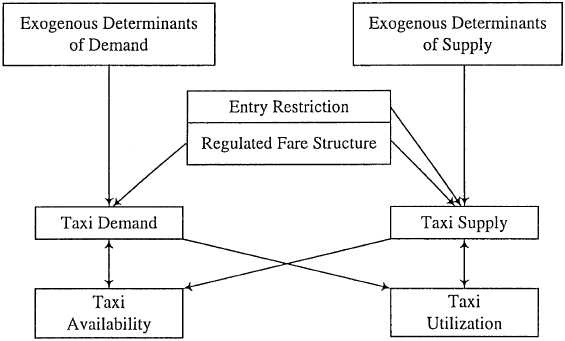
\includegraphics{../figures/taxi_demand}
    \caption{
      Demand-availability-utilization-supply relation in a taxi market. Manski 
      and Wright (1976), cited by \textcite{Yang2002taxi+demand}.
      \label{figure:taxi}
    }
  \end{center}
\end{figure}

Customer demand is modelled as a function of waiting time and fare price in
many studies: \textcite{Douglas1972taxi+regulation, Devany1975taxi+capacity,
Cairns1996taxi+competition, Yang2002taxi+demand} all used customer waiting time
as a proxy for service quality. According to
\textcite{Salanova2011taxi+review}, \textcite{Manski1967taxi+demand} used a
Poisson process (a stochastic function) to simulate demand.

\textcite{Yang2002taxi+demand} use a disaggregate demand model (separately for
each origin-destination pair), where waiting time depends on the number of
vacant taxis in an area near the customer and price depends on the distance
covered; \textcite{Yang2010taxi+nonlinear} added travel time as an additional
variable indicating service quality and assumed that demand decreases as
waiting time increases. \textcite{Yang2010taxi+equilibria} took a slightly
different approach by modelling customer demand as their willingness to pay to
reach a destination, based on their subjective monetary value for using
different modes of transport for reaching a destination; therefore the demand
for taxis in this study was only a part of the total demand for transportation.

\subsection{Reinforcement Learning}
\label{sec:ai}

\subsubsection{Basics}

Reinforecement learning is software agents being rewarded or punished
(receiving negative reward) for their actions so that they can hopefully learn
an optimal policy for acting in some environment, maximising the economic
outcome (\textbf{utility}).

\textbf{Optimal policy} is defined as the mapping of actions from any possible
state to the highest utility outcome from that state. Thus for each state there
is a maximum utility that can be reached. Agents have a set of possible actions
that they can take, depending on the state they are in. Agents also have a set
of rules for what they can observe from the environment. \textbf{Transition
model} is the description of how applying actions to states result in new
states. All of the states, actions and the transition models together define
the \textbf{state space}. \parencite{Russell2010ai+modern,
Sutton1998ai+reinforcement}

\textbf{Reward} is the relative utility (positive or negative) what an agent
gets for being in a certain state, and the goal of the agent is to maximise the
cumulative reward over time. The cumulative reward is known as the
\textbf{value function} or \textbf{utility function}, giving a long-term
outlook in contrast to immediate rewards. Searching and learning the value
function is central to reinforcement learning. \parencite{Russell2010ai+modern,
Sutton1998ai+reinforcement}

Evolutionary methods \parencite{Sutton1998ai+reinforcement} also known as
genetic algorithms \parencite{Russell2010ai+modern} are a branch of artificial
intelligence that could potentially be used for solving reinforcement learning
problems. Evolutionary methods do not learn from individual experiences, and
therefore \textcite{Sutton1998ai+reinforcement} do not recommend using them for
reinforcement learning problems, although they agree that evolutionary methods
could be useful in specific cases. Similarly \textcite{Russell2010ai+modern}
states that genetic algorithms do not cope well with increasing complexity and
are the most useful in optimisation problems.


\subsubsection{Markov Decision Processes}

An agent having the \textbf{Markov property} means that only the current state
of the agent matters to the probability distribution of future states i.e. any
other states and actions do not influence the future state. Even in cases when
the Markov property does not strictly apply, often approximations can be made
and reinforcement learning theory still applies.
\parencite{Sutton1998ai+reinforcement}

A process satisfying the Markov property is a
\textbf{Markov decision process (MDP)}. It consists of the state space and
reward functions. It can be seen that all MDPs have a policy, the one with the
highest expected utility called the \textbf{optimal policy}. It is important to
note that it is the \textit{expected} utility because the environment could be
(and usually is) stochastic. \parencite{Russell2010ai+modern}

Considering MDPs over time, two cases can be distinguished: finite and infinite
horizon. While the optimal action in a given state could change when having a
finite horizon, it never would with an infinite horizon as there is no
differing time pressure. To solve MDPs with an infinite horizon and no terminal
states, rewards need to be discounted. Finding an optimal policy is not always
possible due to the large state space, therefore approximation may be needed.
Approximation can give good results because reaching many states has a very
small probability and they have very low effect on the overall utility of a
policy. \parencite{Russell2010ai+modern}

The simple model of MDPs assumed that the environment was perfectly observable
i.e. the agent knew which state it is in at all times. This assumption is
unrealistic in the real world -- for example, a taxi driver does not know
whether a passenger will accept their offered fare. To account for this,
\textbf{Partially observable Markov decision processes} (POMDP) add the notion
of a \textbf{sensor model} specifying the probabilities of perceiving evidence.
Therefore now the set of states is a set of probability distributions for a
POMDP -- the belief state. \parencite{Russell2010ai+modern}

Therefore it can be concluded that the taxi in the problem in this paper is in a POMDP situation. There is a clear reward function between states - the fare. However, the taxi does not know the exact state it is in i.e. how much the passenger is willing to pay.

\subsubsection{Solving POMDPs}


HEREHEREHERE


\subsubsection{Solving Reinforcement Learning Problems}

Three groups of approaches for solving reinforcement learning problems (finding
optimal policies) are covered by both \textcite{Russell210ai+modern} and
\textcite{Sutton1998ai+reinforcement} can be categorised as follows: model-
free methods (examined in more detail in Section \ref{sec:ai:model_free} and
model-based methods (Section \ref{sec:ai:model_based}). To understand why this
distinction is made, their common background needs to be investigated first.

The simplest naive approach to solve reinforcement learning problems is
\textbf{direct utility estimation}. It uses the fact that utility of a state is
the expected total reward from that state onward, called the reward-to-go.
(Widrow and Hoff, 1960 cited by \textcite{Russell2010ai+modern}) After a large
number of estimations giving samples for the states, the observed reward-to-go
is likely to converge to the actual utility of a state. However, this approach
is inefficient, mainly because it ignores that utilities of states are related
to each other. \parencite{Russell2010ai+modern}

Dynamic programming methods, unlike direct utility estimation, takes in
account the interdependence of utilities of states by learning the transition
model that connects them, and uses dynamic programming to solve the
corresponding Markov decision process. However, this requires a perfectly known
model of the environment which in practice is infeasible. Dynamic programming
is also computationally expensive. The two most popular dynamic programming
methods are value iteration and policy iteration. Dynamic programming is the
basis for both the developed model-based and model-free methods looked at here.
\parencite{Sutton1998ai+reinforcement}

The \textbf{generalized policy iteration} (GPI) (policy iteration ins
\textcite{Russell2010ai+modern}) has been proven to converge to optimal
policies and value functions when using dynamic programming methods. GPI
repeatedly alternates between these two steps: policy evaluation and policy
improvement. Policy evaluation calculates a value function based on the current
policy and updates the existing value function to be closer to the newly
calculated value function. Policy improvement uses the updated value function
to calculate a new policy and then updates the existing policy to be closer to
the newly calculated policy. Most reinforcement learning problems use this
algorithm. \perencite{Sutton1998ai+reinforcement}


\subsubsection{Model-free methods}
\label{sec:ai:model_free}

There are two categories of model-free agents: reflex agents and Q-learning
agents. Q-learning agents learn an action-utility function, giving the expected
utility of taking an action in a given state. Reflex agents learn a policy that
is a direct mapping from states to actions.

Reflex agents are more primitive and 


\subsubsection{Model-based methods}
\label{sec:ai:model_based}


\subsubsection{Temporal difference methods}
\label{sec:ai:temporal}

\textbf{Temporal difference (TD)} does not use a transition model and therefore
is simpler and requires less computation than dynamic programming, alas at a
price of slower learning. TD works by adjusting the utility estimates based on
the differences observed in the last state transition, and over time the
\textit{average} utility values converge to the correct values. To ensure that
utility values in TD converge to the correct value, visited states can be
stored and their repeated impact reduced. \parencite{Russell2010ai+modern}


\subsubsection{Synergy}
\label{sec:ai:synergy}


\newpage
\section{Software and simulation design}
\label{sec:software}
\subsection{Simulation design}
\label{sec:design:simulation}

\subsubsection{Market Considerations}

The approach suggested by this project is not compatible with a market where
fares are regulated, at least in the current form of regulation that specifies
a formula to calculate fares based on some variables, usually time and
distance. Other ways of regulation that do not affect pricing, for example,
market entry conditions, are compatible with the suggested variable pricing
approach.

Three different operational types of taxi markets were introduced in Section
\ref{sec:literature:taxis}: phone-order market, cruising taxi market and taxi
rank market. In the phone-order market and taxi rank customers are actively
seeking a taxi, while in the cruising taxi market passengers can only wait for
a taxi to drive by. Therefore the cruising taxi market is chosen as the easiest
target for simulation, extending it to phone-order and taxi rank markets if the
initial experiment is successful.

The relationship between taxi demand and supply and vice versa was established
in Section \ref{sec:literature:taxis:demand}. This relationship largely depends
on the competitive situation in a taxi market. As the simulation initially
involves only a single taxi, the competition needs to be replicated by other
means. When the simulation is expanded to multiple taxis \textbf{EXTEND}


\subsubsection{Demand: Modelling Passengers}
\label{sec:design:passenger}

Customer demand was reviewed in Section \ref{sec:literature:taxis:demand} where
two approaches to modelling demand were shown: aggregate and disaggregate. An
aggregate demand model "for some portion of the travel market is a function of
variables that describe the product or its consumers"
\parencite{Small2007taxi+urban} The disaggregate approach specifies a set of
variables for each individual passenger. The project goal is investigating taxi
pricing on an individual basis, therefore a disaggregate approach is
preferrable as it allows individual modelling of passengers. \textbf{review
this claim!} Of course, to express demand as a single variable it needs to be
an aggregation of the relevant individual variables.

Therefore each passenger's demand is a function that of some variables. The
different types of variables affecting taxi demand were discussed in Section
\ref{sec:literature:taxis:demand}. Exogenous demand variables are value of time
and value of reliability that can be derived from a passenger's income, hour of
day when travelling, purpose of travel, social status, cost of waiting and
others; these can be modelled for each individual passenger. Taxi availability
is a variable directly depending on the number of vacant taxis in an area, this
is something that passenger's perceive in reality. However, for the simulation,
taxi availability needs to be assumed a constant, at least until machine
learning capabilities are added to passengers and a competitive market
established beyond the very basic simulation, so that passanger agents can
learn the availability on their own.

Let \(P\) be the set of relevant characteristic variables \(c_1,..,c_n\) for a
passenger: \(P = \{c_1,..,c_n\}\), \newline
where each \(c_i : i \in \{1, .., n\}\) has a function \(f_i (c_i) \) that
returns a unity-based normalised value of \(c_i\), \newline
and each \(c_i\) has a weight \(w_i\) representing its relative importance
compared to other variables, where \(\sum_{i=1}^n (w_i) = 1 \). \newline
Then the total probablilstic value \(V(P)\) of a passenger is \[ V(P) =
\sum_{i=1}^{n} (w_i \cdot f_i(c_i) )) \] \newline

Let \(\Delta(o,d)\) be the distance between origin \(o\) to destination \(d\). 
\newline
Let the passenger's expected fare \(F_{expect}\) linearly depend on distance
and a set price \(p\) for a unit of distance. \(F_{expect} = \Delta(o,d) \cdot
p \). \newline
Let the price sensitivity of customers be \(\frac{F_{expect}}{F_{offer}}\). It
is worth noting that a price sensitivity value specific to an individual could
be already included in the passenger characteristics and this is just a global
representation for the whole of system. \newline

Then the probability of a customer accepting a fare \(Q\) for a taxi ride at a
fare price \(F_{offer}\) can be expressed as: 
\begin{equation} 
  \label{eq:design:demand}
  Q_{o \rightarrow d} (P,F_{offer}) = \frac{F_{expect}}{F_{offer}} \cdot V(P)
\end{equation}
This formula is sufficient for the basic case of simulation. It can later be
extended to take in account other determinants of demand as seen in Figure
\ref{figure:taxi} and discussed in Section \ref{sec:literature:taxis:demand}.

The relevant variables for passengers can be generated using a stochastic
process. Similarly, passenger distribution within the network can be generated
using a stochastic process. These processes could take in account some
characteristics observed in reality such as demand variance during the day,
lower passenger income in some areas resulting in lower willingness to pay,
whether a trip is for pleasure or business, and others.


\subsubsection{Taxis in Taxi Market}
\label{sec:design:taxi}

Let taxis have variable costs \(VC\) consisting of driver's wage costs \(w\)
and fuel expenses \(f\), and a sum of fixed costs \(FC\) including e.g.
deprecation, insurance, business overheads, lease payments. For simplicity it
is assumed that wages are paid for all of the time that a taxi is operating,
and a constant amount of fuel costing \(f\) is used for a unit of distance
covered. Then total taxi costs \(TC\) for a total time \(t\) and an amount
total distance covered \(d\) can be expressed as:

\[ TC = VC + FC = t \cdot w + d \cdot f + FC \]

Taxis have a set of available actions. When stopped at a location, they can
decide to drive to another location or wait. If there is a passenger present,
they can start interacting with the passenger, ask for a desired destination
and offer a price.

When taxis interact with customers in reality in a market with no fare
regulation, bargaining is likely to happen: passengers state a destination,
taxis bid passengers a fare, and passengers can agree with it, or decline it
and give a countering bid or abandon the process. Bargaining allows taxis and
passengers to agree on a mutually acceptable price. To simulate real-world
behaviour, a reinforcement learning-based bargaining process can be used as
described in \textcite{Cli1997taxi+bargaining}.

However, sophisticated bargaining can be disregarded in the simulation if the
horizon is significantly long as the agreed fares should converge, albeit at a
slower rate. A simpler approach is limiting the bargaining process to a single
bid which is immediately accepted or declined by the passenger based on the
demand \(Q\). To incentivise the taxi agent, each bid has a cost in time.


\subsubsection{Modelling reinforcement learning}
\label{sec:design:ai}

The research problem needs to be formally defined from a reinforcement learning
point of view according to the definitions in sections \ref{sec:ai:mdp} and
\ref{sec:ai:pomdp}.

It can be assumed that taxi has a complete knowledge of the road network it is
operating in - a realistic assumption given modern GPS navigation systems. In
reality this set would be infinite but it can be simplified to a finite set.
This network forms a part of the total state space. The rest of the state space
is formed of the passenger origin-destination pairs i.e. some state \(s = (o,
d) \). The passenger demand for each of these origin-destination states is
stochastic as mentioned in Section \ref{sec:design:passenger}. 

The actions that a taxi can take were discussed in \ref{sec:design:taxi}. A
simple reward function is as follows. For each moment of time that a taxi is
active, there is an immediate negative reward based on fixed costs and salary
variable costs. If the taxi takes travels, it suffers a negative reward based
on travel variable costs. The only positive reward it gains is from passengers
paying their fares.

If passengers wait at a location for a longer time, then taxis can form
expectations about the possibility of encountering passengers at each location.
To keep track of this uncertainty an agent would need a belief model as
discussed in Section \ref{sec:ai:pomdp}. This complexity can be avoided by
assuming that passengers do not wait for taxis and appear at a location for a
single moment in time only.

\subsubsection{Benchmark} 

To evaluate the variable pricing approach, benchmarks measuring taxi
profitability need to be established using the linear pricing approach. It will
establish the average best-case scenario for both passengers and taxis. If the
reinforcement learning agent can reach or exceed similar profits it will mean
that the experiment was a success.

As noted in \ref{sec:literature:taxis:demand}, the demand and supply
relationship is complex in taxi market. Therefore an equilibrum cannot be
easily calculated and is unlikely to have real value. However, the expected
fare from the Equation \ref{eq:design:demand} linearly depends on distance just
like taxi costs, therefore it is a good indicator for taxi efficiency. The
exact tarriff can be calculated by fixing probability distributions for the
stochastic process and using average values. 

When a tarriff is chosen, the simulation can be run the exact same way as with
a reinforcement learning, the only difference being the agent having no say
about the fare. As the agent faces the same costs in both simulations, costs
need not be taken in account.

\subsubsection{Data}

It is possible to record rewards for each step of time. This data will show
overall profits and reveal how quickly profitability was reached, if at all.

\subsection{Software Design Considerations}

\todo{remove notes}
(10, 2100 w)

Has the student clearly described the design of their system? Is it described
in sufficient detail to make it easy for someone else to replicate the system?

Has the student justified the design decisions, and discussed alternatives that
were considered?


\subsection{Architecture} 
\label{sec:design:architecture}

\todo{consider implementation}

\begin{figure}
  \begin{center}
    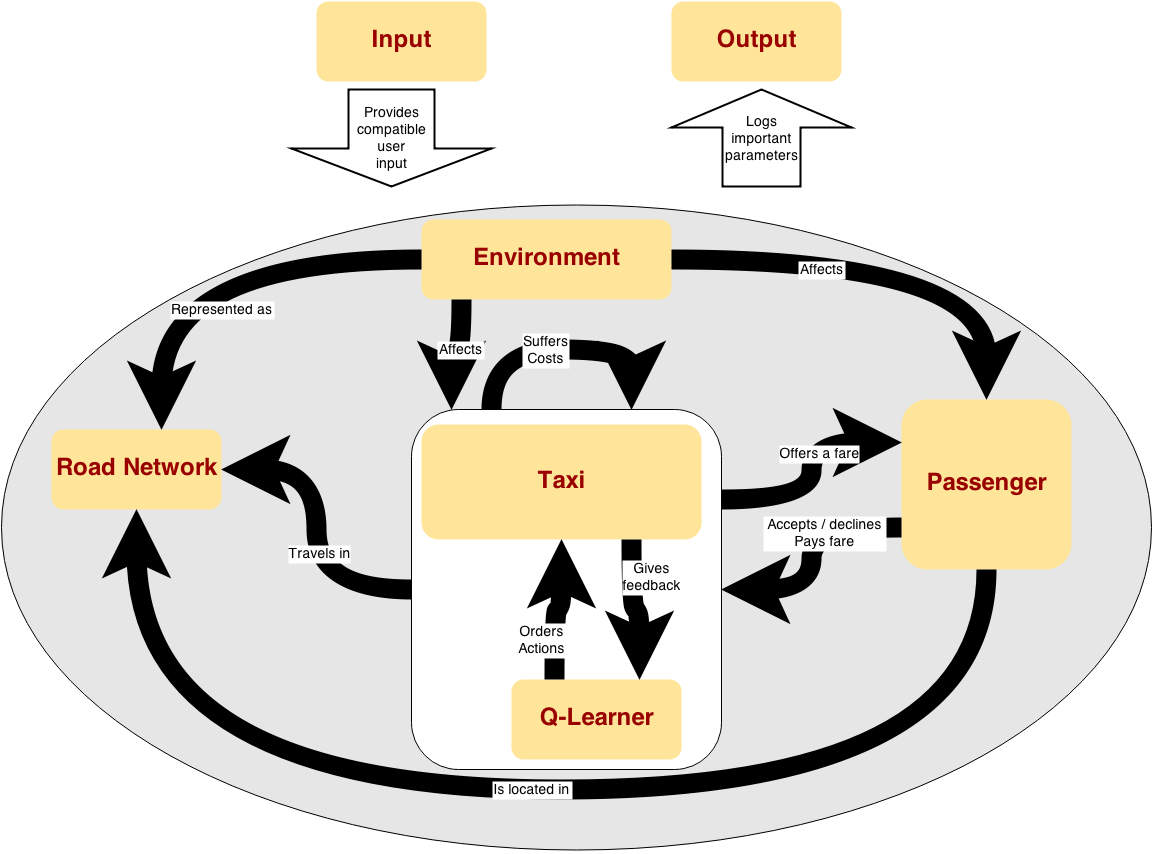
\includegraphics[width=\textwidth]{../figures/software_overview}
    \caption{
      Software overview diagram
      \label{figure:design:software}
    }
  \end{center}
\end{figure}

A software overview diagram is shown in Figure \ref{figure:design:software}.
This section explains the diagram and how the software operates.

When running the simulation, initially some user inputs are processed by the
input module. It validates that the input data (initially parsed from files or
command line parameters) is correct, stopping the program and warning the user
if any invalid data was found. The rest of the system is then initialised
according to the parameters, and a simulation is started.

The environment module is the highest hierarchy simulation object where all
other objects operate in. It is used for keeping track of global variables such
as time and the road network. The environment can directly affect the taxi and
passengers, setting their parameters, and taxis can query the environment for
some information.

The road network is internally represented as a graph, and is where taxis and
passengers are located and interact in.

Passengers (passive agents) can accept or decline taxis' offers respective to
their internal state. If accepted, passengers travel with the taxi in the road
network and pay the agreed fare. Irregardless of the action taken, passengers
disappear after any action is completed.

Taxi (an active agent) is the most complex object in the software. Over time
taxi experiences its own costs (fixed costs and variable costs). Taxis can take
three types of actions: wait at a location, drive to a different location, or
offer a fare to a passenger (if one is present). Taxi's actions are decided by
its learner module. The taxi passes information from the environment to the
learner and receives calls to action. For example, the learner needs to know
what prices it can set (from taxi itself or the environment), what locations it
can drive to (from the road network), whether there is a passenger at the
current location (from the environment), what the passenger's answer to the
offer was (from the passenger).

Finally, there is an output module that logs simulation data to files for
analysis.


\subsection{Technologies}

One of the core technologies used was \textit{git} \parencite{Git} version
control software. Git when used in conjunction with \textit{GitHub}
\parencite{Github} enabled easy code backups to be hosted safely online.
Besides this, commit messages were aimed to be descriptive so that they serve
as a form of documentation of programmer's intentions.

The rest of the technologies used for this project form distinct groups and are
described in the following sections.

\subsubsection{Programming Language}

\textit{Ruby} programming language was chosen as the core technology for this
project due to author's familiarity with it and its related technologies. Ruby
is an object-oriented "dynamic, open source programming language with a focus
on simplicity and productivity. It has an elegant syntax that is natural to
read and easy to write" \parencite{Ruby}.

Ruby has many open-source libraries called \textit{gems} available, hosted and
managed locally by \textit{rubygems} software \parencite{Rubygems}. As these
gems have different versions and depencencies, they need to be managed on a
per-application basis - this process is made easy by \textit{bundler}
\parencite{Bundler}. More on these tools can be found in the Maintenance Manual
in Appendix \ref{sec:maintenance_manual}.

\subsubsection{Cross-Platform Operation and Automation}

Managing different Ruby versions on a single computer can be cumbersome in case
it is needed for multiple Ruby applications. Furthermore, Ruby development for
Windows operating systems (OS) is several months behind development on Unix-
based systems \parencite{Ruby}, rendering the latest versions of Ruby unusable
directly on Windows, at the time of writing including the one this project is
using.

Fortunately, this can easily be avoided by using the following software:
\textit{VirtualBox} \parencite{Virtualbox} virtualisation software to host any
of the most popular OSs, \textit{Vagrant} \parencite{Vagrant} to automatically
manage the OSs and software installed on them, and \textit{RVM} \parencite{Rvm}
to manage Ruby versions on a single OS. Detailed instructions on using this
software stack with Ruby are in the Maintenance Manual in Appendix
\ref{sec:maintenance_manual}. This method also means that the programmer can
easily move between computers as the setup costs are significantly reduced by
automation.


\subsubsection{Supporting Test-Driven Development}
\label{sec:design:software:tdd}

As was explained in Section \ref{sec:design:tdd}, Test-Driven Development (TDD)
is an important method for software development in this project. Therefore
supporting effective TDD is critical. \textit{RSpec} is a TDD testing tool for
Ruby \parencite{Rspec}. The tests are meant to describe the desired behaviour of
software in natural English.

An example RSpec test scenario is shown in Figure \ref{figure:rspec}. This test
specifies behaviour of some ruby class 'Class' which should have a 'currency'
method that returns 'EURO'. If multiple tests are written specifying the
expected behaviour in different conditions, then RSpec tests become a form of
programmer-friendly documentation that is executable and protects the code from
introducing regression bugs.

\begin{figure}
  \begin{verbatim}
    describe Class do
      describe '#currency' do
        it 'is EURO' do
          instance = Class.new
          expect(instance.currency).to eq('EURO')
        end
      end
    end
  \end{verbatim}
  \caption{
    RSpec test example
    \label{figure:rspec}
  }
\end{figure}

RSpec can be enhanced by other tools. \textit{Simplecov} \parencite{Simplecov}
is a code coverage tool that monitors test coverage of a codebase by checking
how many lines of code are executed when running the test suite. \textit{Guard}
\parencite{Guard} is a tool that monitors file changes and executes appropriate
events (i.e. running RSpec tests). This can make a developer's TDD workflow
streamlined leaving with only tests and code to write.


\newpage
\section{Implementation and results}
\label{sec:results}
% (15, 3200 w)

Has the student carried out an evaluation?

Does the student present the results of the evaluation clearly and in a logical
manner?

Does the student explain the problems and difficulties found?

Does the student demonstrate an understanding and interpretation of results and
their significance?

Is there any critical evaluation of the project relative to the achievements of
related works?

Does the student present a personal reflection of what has been achieved and
not achieved in the project?

Has the student suggested future work?


\subsection{Results}
unless noted otherwise, the following inputs were used
 
time limit = 1000000

graph:
  - "0, 1, 2, 4, 2, 1"
  - "1, 0, 2, 2, 3, 0"
  - "2, 2, 0, 0, 1, 3"
  - "4, 2, 0, 0, 1, 0"
  - "2, 3, 1, 1, 0, 5"
  - "1, 0, 3, 0, 5, 0"

passenger: price = 20

taxi: prices = 5..100, benchmark price = 20

Run 1: Non-regulated price much more successful with when the fixed price
equals the expected price. non regulated profit = 1000965; fixed fare loss
-1547613


run: benchmark price = 30

run: benchmark price = 15

run: prices = 5..20

run: prices = 20..100

run: time limit = 50000

\todo{process data and diagrams}

ai profitability over time, see how much time it takes for it to become
profitable etc

look at how the prices charged change over time, if at all


\newpage
\section{Evaluation and discussion}
\label{sec:evaluation}
% (15, 3200 w)

Has the student carried out an evaluation?

Does the student present the results of the evaluation clearly and in a logical
manner?

Does the student explain the problems and difficulties found?

Does the student demonstrate an understanding and interpretation of results and
their significance?

Is there any critical evaluation of the project relative to the achievements of
related works?

Does the student present a personal reflection of what has been achieved and
not achieved in the project?

Has the student suggested future work?


\subsection{Future work}

Software related: fix the shortcomings identified above (TBD); extend to other learners, perhaps even non-MDP based

Socio-economical: evaluate the effect of deregulated prices on
passengers; effective way to model passengers


\newpage
\section{Conclusion}
\label{sec:conclusion}
% \newpage
\section{Conclusion}
\label{sec:conclusion}

This project was mostly successful in implementing a software simulation of a
taxi market where fare prices are chosen by a Q-Learner agent. 

The software fulfilled all of the core goals to the minimum specification, and
exceeded the minimum requirements in some areas. The software suffers from
several small implementation issues that have been clearly identified, and a
plan for fixing these issues was provided. While some problems were identified
with the software development approach that was followed, it was adequate and
proved beneficial overall.

The simulation experiment was successfully completed with six different
scenarios, testing different aspects of the system. It was found that having
variable fare pricing results in significantly larger profits to a taxi.
Furthermore, it was clear that the Q-Learner was a reasonable choice for
controlling the taxi and it's fare pricing as it showed a clear trend of
increasing profits over time.

However, the results additionally revealed an inconclusive profitability trend
for the Q-Learner in the fixed pricing simulation scenarios conducted for
benchmarking. This suggests that there may be a bug or a design oversight in
the software which will need fixing in future.

Nevertheless, variable pricing proved to be more profitable than fixed pricing,
therefore opening future possibilities for the project's topic and software.
Possible future work includes fixing the known issues with the software,
experimenting with different reinforcement learning strategies or even
researching the wider social implications of a variable fare pricing approach.
Beyond the realm of taxis, it is worth considering to utilise variable pricing
and reinforcement learning for public transport in general.


\newpage
\printbibliography

\end{document}